\renewcommand{\lastmod}{20. Dezember 2024}
\renewcommand{\chapterauthors}{Markus Lippitz}

\chapter{Schwingung in Molekülen}



\section{Überblick} 


% In diesem Kapitel behandeln wir die Spektroskopie von Molekülen mit dem Ziel, die Eigenschaften des Bindungspotentials zu bestimmen. Wir beginnen mit einem allgemeinen, spektral sehr breiten Überblick über die spektroskopischen Eigenschaften von Molekülen, die in ihren dielektrischen Eigenschaften zum Ausdruck kommen. Die dielektrische 'Konstante' kann als eine Summe von Lorentz-Oszillatoren dargestellt werden.  Jeder Oszillator, jede Resonanz entspricht einem Freiheitsgrad des Moleküls. In diesem Kapitel werden Rotationen und Schwingungen behandelt, im nächsten Kapitel die elektronische Anregung. Elektronische Anregung ist die Anregung, die wir schon bei den Atomen besprochen haben. Aber nur Moleküle, die aus mehr als einem Atom bestehen, können gegeneinander schwingen oder sich drehen.

% Der zweite Abschnitt dieses Kapitels befasst sich daher mit den Rotationen der Moleküle und wie sie sich im Spektrum widerspiegeln. Wir werden sehen, dass Rotationen im Modell des starren Rotators zu einer Reihe von äquidistanten Linien mit einer charakteristischen Amplitudenverteilung führen.

Ein schwingendes Molekül zeigt zunächst nur eine Linie im Spektrum. In Kombination mit der Rotation entstehen jedoch weitere Linien, wenn sich bei einem optischen Übergang die Rotationsquantenzahl und die Schwingungsquantenzahl gleichzeitig ändern. Schließlich versuchen wir, die Vielzahl möglicher Schwingungen in mehratomigen Molekülen zu beschreiben.


\begin{figure}
\inputtikz{\currfiledir fig_hcn-single}
\caption{Infrarot-Absorptionsspektrum von \ch{HCN}-Gas  (\cite{Maki_1995_HCN} via \href{https://hitran.org}{hitran.org}).
\label{fig:vib_hcn}}
\end{figure}

%other sources 
%https://webbook.nist.gov/cgi/cbook.cgi?ID=C74884&Type=IR-SPEC&Index=1#IR-SPEC



Absorptionsspektren in diesen (Nah-)Infraroten Wellenlängenbereich misst man beispielsweise durch Fourier-Transformations-Infrarot-Spektroskopie (FTIR). Als Lichtquelle wird oft ein breitbandiger Infrarotstrahler benutzt, der aus einem Silizium-Carbid-Stab (Globar) besteht, durch den ein Strom fließt und so heizt. Das durch die Probe transmittierte Licht wird durch ein Michelson-Interferometer geleitet und mit einem infrarot-  also Wärme-empfindlichen Detektor (Bolometer) gemessen. Dieser Detektor selbst kann nur die Gesamt-Intensität messen. Das Michelson-Interferometer wirkt aber als spektraler Filter mit einer sinusförmigen Transmission. Die Periode der spektralen Modulation wird über den Armlängen-Unterschied eingestellt und kontinuierlich variiert. Aus der Fourier-Transformation der gemessenen Intensität als Funktion des Armlängen-Unterschieds erhält man das Spektrum des Infrarot-Lichts, also Intensität als Funktion der Wellenlänge.



\section{Harmonische Näherung des Bindungspotentials}

\begin{marginfigure}
\inputtikz{\currfiledir vib_state_wf}
\caption{Die Eigenfunktionen des quantenmechanischen harmonischen Oszillators für $\nu = 0 \dots 5$ (dünne Linie) und die Aufenthaltswahrscheinlichkeit (gefüllte Kurven). Die Position in y-Richtung entspricht der Eigen-Energie des Zustands auf der Skala des parabelförmigen Bindungspotentials im Hintergrund.
\label{fig:vib_1d_WF}}
\end{marginfigure}

In der Nähe des Minimums, rund um den Gleichgewichtsabstand $R_0$ lässt sich das Bindungspotential sicherlich als harmonisches Potential im Kern-Kern-Abstand $R$ nähern. Wir machen also die Annahme für das Bindungspotential $U(R)$
\begin{equation}
U(R)  = \frac{1}{2} \, k \, (R - R_0 )^2 = \frac{1}{2} \, k \, r^2 
\end{equation}
mit der Federkonstanten $k = \mu \, \omega_0^2$ und der Auslenkung $r$ aus dem Gleichgewicht. Die Wellenfunktionen und Energie-Eigenwerte in solch einem Potential hatten wir uns schon im den einführenden Kapiteln zur Quantenmechanik angeschaut.
Die Schwingungs-Wellenfunktion des eindimensionalen harmonischen Oszillators sind
\begin{equation}
\Psi_\text{vib} =  U(\xi) = \left(\frac{\mu \omega_0}{\pi \hbar} \right)^{\frac{1}{4}} \,
 H_\nu(\xi) \, e^{- \xi^2 /2}
\end{equation}
mit den Hermite'schen Polynomen $H_\nu(\xi)$.
Die Energie-Eigenwerte sind
\begin{equation}
E_\nu = \hbar \omega_0 \left(\nu + \frac{1}{2} \right) \quad \text{mit} \quad \nu = 0, 1, 2 \dots
\end{equation}
und $\omega_0 = \sqrt{k / \mu}$.



\section{Auswahlregeln für reine Schwingungsübergänge}

Lässt sich die Schwingung eines Moleküls (eigentlich der Kerne entlang der Bindungsachse) durch die Absorption eines Photons anregen? Oder andersherum: hinterlassen die Schwingungs-Energie-Eigenwerte $E_\nu$ von oben einen beobachtbaren Effekt? Hier wollen wir uns darauf beschränken, \emph{nur} die Schwingung anzuregen. Weiter unten werden wir Kombinationen mit anderen Anregungen (Rotation, elektronisch) diskutieren.

Um diese Fragen zu beantworten, brauchen wir wie im Kapitel zur Wechselwirkung mit Licht das  Übergangsdipolmoment $\mathbf{D}_{fi}$ 
\begin{equation}
 \mathbf{D}_{fi} = \braket{f | \hat{\mu} | i} 
\end{equation}
und den Dipol-Operator $\hat{\mu}= e \hat{\br}$. Die Auswahlregeln beantworten die Frage, unter welchen Umständen dieser Term nicht Null ist. Die absolute Größe interessiert uns hier also nicht so sehr.


Dazu brauchen wir eigentlich  die Kern-Wellenfunktionen, die also die Aufenthaltswahrscheinlichkeit der beiden Kerne beschrieben. Das beinhaltet alle Bewegung der Kerne, Rotation und Schwingung. Für die Schwingung alleine reicht der Radialanteil, genau das $\Psi_\text{vib}$, was wir oben beim Parabeipotential gefunden hatten.
 Genauso besteht der Dipol-Operator eigentlich aus der Summe über alle Ladungen mal deren Ortsvektor. Auch dies vereinfacht sich zu dem Radialanteil der Kernladungen $d_k(R)$. Weiterhin nähern wir den Operator in einer Taylor-Reihe um $R \approx R_0$ und behalten nur das erste Glied. Die vollständige Rechnung findet sich in Kapitel 4.2 von \cite{Demtröder_molekuelphysik}. Dabei verschwindet auch das nullte Glied der Taylor-Reihe, das das statische Dipolmoment beschreibt. Man findet schließlich, dass das Übergangsmatrixelement gegeben ist durch
\begin{equation}
D_{fi}^\text{vib} \propto  \left. \frac{\partial d_k}{\partial R} \right|_{R_0} \,  \int (\Psi_\text{vib}^\star (R) )_f \, R  \, \, (\Psi_\text{vib} (R) )_i \, dR \quad .
\end{equation}
Reine Schwingungsübergang sind also nur dann erlaubt, wenn sich das permanente Dipolmoment mit dem Kern-Kern-Abstand ändert. Solche Moleküle werden \emph{infrarotaktiv} genannt. Dann  darf auch das Integral nicht verschwinden. Aufgrund einer Eigenschaft der Hermite'schen Polynome ist das nur dann der Fall, wenn sich die Quantenzahl $\nu$ zwischen den beiden Zuständen nur um eins unterscheidet, also 
\begin{equation}
 \Delta \nu = \pm 1 \quad .
\end{equation}
Reine Schwingungsübergänge sind also nur zwischen benachbarten Zuständen möglich, und das auch nur für manche Moleküle, bei denen sich das Dipolmoment mit dem Kern-Kern-Abstand ändert. \ch{NO} ist also infrarotaktiv, \ch{H2} nicht. Da im harmonischen Oszillator die Zustände äquidistant sind, bestehen reine Schwingungsspektren in diesem Fall aus einer einzigen Linie bei 
\begin{equation}
 \bar{\nu}_\text{vib} = \frac{\hbar \omega_0}{h c} = \frac{\sqrt{k / \mu} }{2 \pi  c} \quad .
\end{equation}

Das oben gezeigte Spektrum ist deutlich komplexer. Unsere Annahme, dass sich allein die Schwingungs-Quantenzahl $\nu$ ändert, ist also (zu) weitreichend. Es wird sich zeigen, dass der scharfe Peak bei $\bar{\nu} = 715$~cm$^{-1}$ ein reiner Schwingungsübergang ist.

\section{Anharmonisches Bindungspotential}

Die harmonische Parabel ist nur eine erste Näherung für das Bindungspotential. Man kann verschiedene, besser zutreffende analytische Potentiale aufstellen. Oft wird das \emph{Morse-Potential} verwendet, weil auch mit ihm  die Schrödinger-Gleichung exakt lösbar ist. Das Potential hat die Form
\begin{equation}
 V(R) = D_e \left( 1 - e^{-a (R - R_0)} \right)^2 \approx D_e \, a^2 (R - R_0)^2 + \cdots \quad .
\end{equation}
Dabei ist $D_e$ die Dissoziationsenergie des Moleküls, also die Tiefe des Minimums unter der Energie bei $R \rightarrow \infty$. In der harmonischen Näherung des Morse-Potentials entspricht $k = 2 D_e a^2$ der Federkonstanten bzw. $\omega_0 = a \sqrt{2 D_e / \mu}$ der Eigenfrequenz. In diesem anharmonischen Potential  sind die Energien nicht mehr äquidistant. Die Abstände zwischen benachbarten Zuständen nehmen mit steigender Quantenzahl $\nu$ ab. Die Auswahlregeln werden auch aufgeweicht, und Übergänge mit 
\begin{equation}
\Delta \nu = \pm 1, \pm 2 , \pm 3, \dots
\end{equation}
werden erlaubt, wenn auch sie mit steigendem $|\Delta \nu |$ schnell schwächer werden. Der spektroskopisch sichtbare Effekt des anharmonischen Bindungspotentials sind also die Obertöne, also Linien bei in etwa ganzzahligen Vielfachen der harmonischen Linie. Die Aufspaltung der harmonischen Linie selbst ist deutlich schwieriger zu beobachten. Für CO beispielsweise liegt der Grundton bei $\bar{\nu}_1 = 2142$~cm$^{-1}$ und der erste Oberton bei 
 $\bar{\nu}_2 = 4269$~cm$^{-1}$, aber $2 \bar{\nu}_1 = 4284$~cm$^{-1}$.
 
\begin{marginfigure}
\inputtikz{\currfiledir fig_vib_states}
\caption{Zustände und Übergange im harmonischen und anharmonischen Oszillator.}
\end{marginfigure}
 
 
 
Das anharmonische Bindungspotential erklärt auch die Expansion von Festkörpern --- eigentlich ein Thema für das nächste Semester. Der Schwerpunkt der Aufenthaltswahrscheinlichkeit der Schwingungs-Wellenfunktionen verschiebt sich mit steigender Quantenzahl im anharmonischen Oszillator zu größeren Bindungsabständen. Im harmonischen Oszillator bleibt er immer beim Gleichgewichtsabstand. Mit höherer Temperatur werden also immer höhere Schwingungszustände besetzt und so dehnt sich Materie aus.


\section{Rotation und Schwingung gleichzeitig}

Nun soll auch die Rotation des Moleküls erlaubt sein. Wir gehen hier davon aus, dass diese beiden Bewegungen sich nicht gegenseitig beeinflussen, also nicht gekoppelt sind. Die Energie-Eigenwerte sind dann gerade die Summe der Zustandsenergien aus Rotation und Schwingung%\sidenote{Wir nehmen hier einen harmonischen Oszillator und einen starren Rotator an!}
\begin{equation}
E (\nu, J) = E_\text{vib}(\nu) + E_\text{rot}(J) = \hbar \omega_0 \left(\nu + \frac{1}{2} \right) + h c \, B J \left( J+1 \right) \label{eq:vib_rot_simple}
\end{equation}
mit der Rotations-Quantenzahl $J$ und der Vibrations-Quantenzahl $\nu$. Der energetische Abstand der Vibrationszustände ist mit etwa $1000$~cm$^{-1}$  größer als der der Rotationszustände mit etwa $100$~cm$^{-1}$. Man kann sich also vorstellen, dass nun jeder Schwingungszustand mit einer Sequenz von Rotationszuständen dekoriert ist.

Die Auswahlregeln sind zunächst dieselben wie wir sie bereits für die beiden Prozesse separat diskutiert hatten. Hinzu kommt die Möglichkeit, dass nichts passiert, also sich nur die andere Quantenzahl verändert. Damit haben wir
\begin{equation}
 \Delta \nu = 0, \pm 1 \quad \text{und} \quad \Delta J = 0, \pm 1  \quad ,
\end{equation}
aber nicht alle Kombinationen sind möglich oder interessant.

\paragraph{Nichts passiert} Der Fall $\Delta \nu = \Delta J = 0$ ist langweilig.

\paragraph{Reine Rotationsübergänge} Falls $\Delta \nu = 0$ ändert sich nur der Rotationszustand. Dies ist die Situation, die wir im am Anfang des Kapitel besprochen haben, und führt zu Linien  in einem anderen Spektralbereich, bei etwa $\bar{\nu} \approx 100$~cm$^{-1}$.

\paragraph{Reine Schwingungsübergänge} Oben haben wir den  harmonischen Oszillator betrachtet unter der Annahme $J=0$. Dies schließt $\Delta J = 0$ mit ein. Bei einem von Null verschiedenen $J$ muss sich dieses aber bei einem Schwingungsübergang ändern, zumindest für eine zweiatomiges Molekül. Eine höhere Schwingungsanregung ändert den mittleren Kern--Kern--Abstand und somit das Trägheitsmoment. Die Drehimpulserhaltung verlangt dann, dass sich die Rotationsquantenzahl $J$ ändert. $\Delta J = 0$ ist also verboten für einfache, zu symmetrische Moleküle, andernfalls erlaubt. Wenn diese Übergänge erlaubt sind, dann führen sie zu einer einzigen Linie im Spektrum bei $ \bar{\nu}_0 = (\hbar \omega_0)/(h c) $, analog dem reinen Schwingungsspektrum. Diese wird 'Q-Zweig' genannt. 

\paragraph{P-Zweig} Falls $\Delta J = -1$ ist, und $\Delta \nu = +1$ (in Absorption eines IR Photons) oder $-1$ (in Emission eines IR Photons), dann führen diese Übergänge zum sogenannten P-Zweig. Die Linienpositionen sind
\begin{equation}
 \frac{\Delta E}{h c} = \frac{1}{h c} \left( E(\nu +1, J -1) - E(\nu, J) \right) = \frac{\hbar \omega_0}{h c}   - 2 B J \quad .
\end{equation}
Wir erhalten also eine äquidistante Schar von Linien, völlig analog dem reinen Rotationsspektrum, insbesondere auch im dort besprochenen Verlauf der Amplituden. Der einzige Unterschied ist das negative Vorzeichen. Die Linienschar ist also gespiegelt gegenüber dem THz-Spektrum und beginnt an der reinen Schwingungslinie $\bar{\nu}_0 $.

\paragraph{R-Zweig} Analog zum P-Zweig, nur mit  $\Delta J = +1$ nur mit den Linienpositionen
\begin{equation}
 \frac{\Delta E}{h c} =  \bar{\nu}_0   + 2 B ( J +1)
\end{equation}
also in der gleichen Orientierung wie das THz-Spektrum und bei $\bar{\nu}_0 $ beginnend.

Mit diesen Überlegungen können wir das in Abbildung \ref{fig:vib_hcn} gezeigte Spektrum zumindest qualitativ erklären.


\begin{marginfigure}
\inputtikz{\currfiledir rot_vib}
\caption{Rotations-Vibrations-Übergänge liefert die P, Q, R-Zweige im Spektrum.}
\end{marginfigure}
 
 



\section{Mehratomige Moleküle}

Wenn ein Molekül aus mehr als zwei Atomen besteht, dann gibt es viele verschiedene, komplexe Muster der Auslenkung der einzelnen Atome aus ihrer Gleichgewichtsposition. Es gibt also mehr als eine Schwingungsmode in solchen Molekülen.

Die Anzahl der Schwingungsmoden lässt sich aus der Summe der Freiheitsgrade berechnen. Bei $N$ Atomen im Molekül hat jedes Atom $3$ Translations-Freiheitsgrade\sidenote{Atome sind hier punktförmig, können also nicht rotieren und haben daher keine Rotationsfreiheitsgrade}. Diese insgesamt $3N$ Freiheitsgrade müssen auch im Molekül existieren. Sie lassen sich aufteilen in
\begin{itemize} \setlength{\itemsep}{0pt}
\item Schwerpunktbewegung: 3 Freiheitsgrade
\item Rotation des Moleküls: 2 Freiheitsgrade, falls lineares Molekül, sonst 3 Freiheitsgrade
\item Schwingung: der ganze Rest, also $3N-5$ für ein lineares Molekül bzw. $3N-6$ für alle anderen Moleküle. 
\end{itemize}

Ein zweiatomiges Molekül wie beispielsweise \ch{H2} muss linear sein, hat also nur einen Schwingungs-Freiheitsgrad. Ein dreiatomiges Molekül kann linear sein, wie \ch{CO2} und hat dann 4  Schwingungs-Freiheitsgrade, oder es ist nicht gerade, wie \ch{H2O}, und hat dann nur 3  Schwingungs-Freiheitsgrade. Naphthalin beispielsweise besteht aus $N=18$ Atomen und hat damit  48 Schwingungs-Freiheitsgrade. Das Konzept der Normalmoden\sidenote{siehe beispielsweise Kapitel 6.3 in \cite{Demtröder_molekuelphysik}} aus der Mechanik erlaubt hier den Überblick zu behalten.

\section{Beispiele}

Wie kommt man an die Normalmoden? Einen systematischen Weg bietet die Betrachtung der Symmetrie der Moleküle, die sich in der Symmetrie der Normalmoden widerspiegeln muss. Dies geschieht im Rahmen der Gruppentheorie, die hier allerdings zu weit gehen würde.\sidenote{Mehr dazu in einer Vorlesung zur Kristallografie, oder qualitativ in \cite{Atkins}.} Hier raten wir einfach. Dabei hilft es, vorher auszurechnen, wie viele Moden man finden muss, also wie viele Schwingungsfreiheitsgrade es gibt. Auch sollte sich dabei der Schwerpunkt nicht bewegen, oder das ganze Molekül sich drehen, weil das ja separat behandelt wird.

\paragraph{Kohlendioxid} 
Ein lineares Molekül mit $f=9 - 5 = 4$ Schwingungsfreiheitsgraden


\begin{description}
\item[Symmetrische Streckschwingung]
\begin{marginfigure}
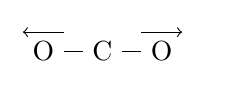
\begin{tikzpicture}
\useasboundingbox (-0.2,-0.2) rectangle (2,0.3);
%\draw (-0.2,-0.2) rectangle (2,0.3);

\draw  (0,0) node (o1) {O};
\draw  (0.75,0) node (c) {C};
\draw  (1.5,0) node (o2) {O};

\draw (o1) -- (c) -- (o2);
\draw[->] (o1.north east) -- (o1.north west);
\draw[<-] (o2.north east) -- (o2.north west);
\end{tikzpicture}
\end{marginfigure}
  $\bar{\nu} = 1337$~cm$^{-1}$. Hierbei ändert sich das Dipolmoment nicht, die Schwingung ist also nicht IR aktiv, wäre im Spektrum also nicht zu sehen.


\item[Asymmetrische Streckschwingung]
\begin{marginfigure}
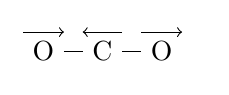
\begin{tikzpicture}
\useasboundingbox (-0.2,-0.2) rectangle (2,0.3);
%\draw (-0.2,-0.2) rectangle (2,0.3);

\draw  (0,0) node (o1) {O};
\draw  (0.75,0) node (c) {C};
\draw  (1.5,0) node (o2) {O};

\draw (o1) -- (c) -- (o2);
\draw[<-] (o1.north east) -- (o1.north west);
\draw[<-] (o2.north east) -- (o2.north west);
\draw[->] (c.north east) -- (c.north west);
\end{tikzpicture}
\end{marginfigure}
 $\bar{\nu} = 2349$~cm$^{-1}$. Hierbei ändert sich das Dipolmoment, die Schwingung ist also  IR aktiv.

\item[Biegeschwingung] 
\begin{marginfigure}
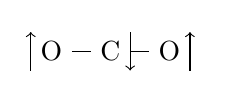
\begin{tikzpicture}
\useasboundingbox (-0.3,-0.2) rectangle (2,0.3);
%\draw (-0.2,-0.2) rectangle (2,0.3);

\draw  (0,0) node (o1) {O};
\draw  (0.75,0) node (c) {C};
\draw  (1.5,0) node (o2) {O};

\draw (o1) -- (c) -- (o2);
\draw[<-] (o1.north west) -- (o1.south west);
\draw[<-] (o2.north east) -- (o2.south east);
\draw[->] (c.north east) -- (c.south east);
\end{tikzpicture}
\end{marginfigure}
 $\bar{\nu} = 667$~cm$^{-1}$. Hierbei ändert sich das Dipolmoment, die Schwingung ist also  IR aktiv. Diese Mode ist zweifach entartet, da sie auch in der Ebene senkrecht zum Papier schwingen könnte. Für die Biegung ist das Potential weicher, die Frequenz daher niedriger als für die Streckung.
\end{description}


\paragraph{Wasser} Ein nicht-lineares Molekül mit $f=9 - 6 = 3$ Schwingungsfreiheitsgraden
\begin{description}
\item[Symmetrische Streckschwingung] 
\begin{marginfigure}
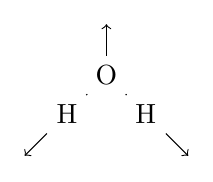
\begin{tikzpicture}
\useasboundingbox  (-0.5,-0.5) rectangle (1.5,1.1);
%\draw (-0.5,-0.5) rectangle (1.5,1.1);

\draw  (0,0) node (h1) {H};
\draw  (0.5,0.5) node (o) {O};
\draw  (1,0) node (h2) {H};

\draw (h1) -- (o) -- (h2);
\draw[->] (h1.south west) -- ++(-135:4mm);
\draw[->] (h2.south east) -- ++(-45:4mm);
\draw[->] (o.north) -- ++(up:4mm);
\end{tikzpicture}
\end{marginfigure}
  $\bar{\nu} = 3657$~cm$^{-1}$. Hierbei ändert sich das Dipolmoment, die Schwingung ist also  IR aktiv.

\item[Symmetrische Streck-Biegeschwingung]
\begin{marginfigure}
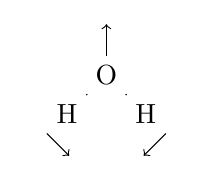
\begin{tikzpicture}
\useasboundingbox  (-0.5,-0.5) rectangle (1.5,1.1);
%\draw (-0.5,-0.5) rectangle (1.5,0.75);

\draw  (0,0) node (h1) {H};
\draw  (0.5,0.5) node (o) {O};
\draw  (1.,0) node (h2) {H};

\draw (h1) -- (o) -- (h2);
\draw[->] (h1.south west) -- ++(-45:4mm);
\draw[->] (h2.south east) -- ++(-135:4mm);
\draw[->] (o.north) -- ++(up:4mm);
\end{tikzpicture}
\end{marginfigure}
  $\bar{\nu} = 1595$~cm$^{-1}$. Hierbei ändert sich das Dipolmoment, die Schwingung ist also  IR aktiv.

\item[Asymmetrische Schwingung]
\begin{marginfigure}
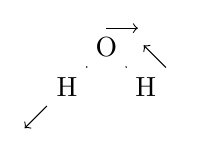
\begin{tikzpicture}
\useasboundingbox  (-0.5,-0.5) rectangle (1.5,0.75);
%\draw (-0.5,-0.5) rectangle (1.5,0.75);

\draw  (0,0) node (h1) {H};
\draw  (0.5,0.5) node (o) {O};
\draw  (1.,0) node (h2) {H};

\draw (h1) -- (o) -- (h2);
\draw[->] (h1.south west) -- ++(-135:4mm);
\draw[->] (h2.north east) -- ++(135:4mm);
\draw[->] (o.north) -- ++(east:4mm);
\end{tikzpicture}
\end{marginfigure}
  $\bar{\nu} = 3756$~cm$^{-1}$. Hierbei ändert sich das Dipolmoment, die Schwingung ist also  IR aktiv.
  
  
\end{description}

\begin{figure}
\inputtikz{\currfiledir fig_hcn-lowres}
\caption{Infrarot-Absorptionsspektrum von HCN Gas  (\cite{Maki_1995_HCN} via \href{https://hitran.org}{hitran.org}). Im unteren Spektrum ist ein größerer Ausschnitt bei geringer Auflösung gezeigt. Hier sind von den Rotationsbanden nur die Einhüllenden zu erkennen.
\label{fig:vib_hcn_all}}
\end{figure}


\paragraph{Cyanwasserstoff (Blausäure, HCN)}  
\begin{marginfigure}
\inputtikz{\currfiledir fig_hcn_modes}
\end{marginfigure}
Ein lineares Molekül mit $f=9 - 5 = 4$ Schwingungsfreiheitsgraden, analog zu Kohlendioxid oben. Das Spektrum in Abb. \ref{fig:vib_hcn} weiter oben zeigt die Biegeschwingung bei $\bar{\nu} = 712$~cm$^{-1}$.  Abbildung \ref{fig:vib_hcn_all} gibt einen Überblick über einen größeren Spektralbereich. Man sieht zusätzlich den 
ersten Oberton der Biegeschwingung bei ungefähr der doppelten Frequenz  $\bar{\nu} = 1415$~cm$^{-1}$. Die Mode bei  $\bar{\nu} = 3312$~cm$^{-1}$ ist die  asymmetrische Streckschwingung. Die symmetrische Streckschwingung  bei $\bar{\nu} = 2114$~cm$^{-1}$.
 Im Gegensatz zu \ch{CO2} bewegt sich in dieser Mode das Kohlenstoffatom ebenfalls, da die Massen von H und N verschieden sind, und sich ansonsten der  Schwerpunkt bewegen würde. Dies macht diese Mode sehr schwach IR-aktiv.  Nur für den Grundton der Biegeschwingung und die  symmetrische Streckschwingung ist der Q-Zweig erlaubt.




%%%%%%%%%%%%%%%%%%%%%%%%%%%%%%%%%%%%%%%%



\section{Zusammenfassung}

\textit{Schreiben Sie hier ihre persönliche Zusammenfassung des Kapitels auf. Konzentrieren Sie sich auf die wichtigsten Aspekte.}

\vspace*{10cm}


%--------------------
\printbibliography[segment=\therefsegment,heading=subbibliography]
